\documentclass[a4paper,12pt,twoside]{memoir}

% Castellano
\usepackage[spanish,es-tabla]{babel}
\selectlanguage{spanish}
\usepackage[utf8]{inputenc}
\usepackage[T1]{fontenc}
\usepackage{lmodern} % Scalable font
\usepackage{microtype}
\usepackage{placeins}

\RequirePackage{booktabs}
\RequirePackage[table]{xcolor}
\RequirePackage{xtab}
\RequirePackage{multirow}

% Links
\PassOptionsToPackage{hyphens}{url}\usepackage[colorlinks]{hyperref}
\hypersetup{
	allcolors = {red}
}

% Ecuaciones
\usepackage{amsmath}

% Rutas de fichero / paquete
\newcommand{\ruta}[1]{{\sffamily #1}}

% Párrafos
\nonzeroparskip

% Huérfanas y viudas
\widowpenalty100000
\clubpenalty100000

% Imagenes
\usepackage{graphicx}
\newcommand{\imagen}[2]{
	\begin{figure}[!h]
		\centering
		\includegraphics[width=0.9\textwidth]{#1}
		\caption{#2}\label{fig:#1}
	\end{figure}
	\FloatBarrier
}

\newcommand{\imagenflotante}[2]{
	\begin{figure}%[!h]
		\centering
		\includegraphics[width=0.9\textwidth]{#1}
		\caption{#2}\label{fig:#1}
	\end{figure}
}



% El comando \figura nos permite insertar figuras comodamente, y utilizando
% siempre el mismo formato. Los parametros son:
% 1 -> Porcentaje del ancho de página que ocupará la figura (de 0 a 1)
% 2 --> Fichero de la imagen
% 3 --> Texto a pie de imagen
% 4 --> Etiqueta (label) para referencias
% 5 --> Opciones que queramos pasarle al \includegraphics
% 6 --> Opciones de posicionamiento a pasarle a \begin{figure}
\newcommand{\figuraConPosicion}[6]{%
  \setlength{\anchoFloat}{#1\textwidth}%
  \addtolength{\anchoFloat}{-4\fboxsep}%
  \setlength{\anchoFigura}{\anchoFloat}%
  \begin{figure}[#6]
    \begin{center}%
      \Ovalbox{%
        \begin{minipage}{\anchoFloat}%
          \begin{center}%
            \includegraphics[width=\anchoFigura,#5]{#2}%
            \caption{#3}%
            \label{#4}%
          \end{center}%
        \end{minipage}
      }%
    \end{center}%
  \end{figure}%
}

%
% Comando para incluir imágenes en formato apaisado (sin marco).
\newcommand{\figuraApaisadaSinMarco}[5]{%
  \begin{figure}%
    \begin{center}%
    \includegraphics[angle=90,height=#1\textheight,#5]{#2}%
    \caption{#3}%
    \label{#4}%
    \end{center}%
  \end{figure}%
}
% Para las tablas
\newcommand{\otoprule}{\midrule [\heavyrulewidth]}
%
% Nuevo comando para tablas pequeñas (menos de una página).
\newcommand{\tablaSmall}[5]{%
 \begin{table}
  \begin{center}
   \rowcolors {2}{gray!35}{}
   \begin{tabular}{#2}
    \toprule
    #4
    \otoprule
    #5
    \bottomrule
   \end{tabular}
   \caption{#1}
   \label{tabla:#3}
  \end{center}
 \end{table}
}

%
% Nuevo comando para tablas pequeñas (menos de una página).
\newcommand{\tablaSmallSinColores}[5]{%
 \begin{table}[H]
  \begin{center}
   \begin{tabular}{#2}
    \toprule
    #4
    \otoprule
    #5
    \bottomrule
   \end{tabular}
   \caption{#1}
   \label{tabla:#3}
  \end{center}
 \end{table}
}

\newcommand{\tablaApaisadaSmall}[5]{%
\begin{landscape}
  \begin{table}
   \begin{center}
    \rowcolors {2}{gray!35}{}
    \begin{tabular}{#2}
     \toprule
     #4
     \otoprule
     #5
     \bottomrule
    \end{tabular}
    \caption{#1}
    \label{tabla:#3}
   \end{center}
  \end{table}
\end{landscape}
}

%
% Nuevo comando para tablas grandes con cabecera y filas alternas coloreadas en gris.
\newcommand{\tabla}[6]{%
  \begin{center}
    \tablefirsthead{
      \toprule
      #5
      \otoprule
    }
    \tablehead{
      \multicolumn{#3}{l}{\small\sl continúa desde la página anterior}\\
      \toprule
      #5
      \otoprule
    }
    \tabletail{
      \hline
      \multicolumn{#3}{r}{\small\sl continúa en la página siguiente}\\
    }
    \tablelasttail{
      \hline
    }
    \bottomcaption{#1}
    \rowcolors {2}{gray!35}{}
    \begin{xtabular}{#2}
      #6
      \bottomrule
    \end{xtabular}
    \label{tabla:#4}
  \end{center}
}

%
% Nuevo comando para tablas grandes con cabecera.
\newcommand{\tablaSinColores}[6]{%
  \begin{center}
    \tablefirsthead{
      \toprule
      #5
      \otoprule
    }
    \tablehead{
      \multicolumn{#3}{l}{\small\sl continúa desde la página anterior}\\
      \toprule
      #5
      \otoprule
    }
    \tabletail{
      \hline
      \multicolumn{#3}{r}{\small\sl continúa en la página siguiente}\\
    }
    \tablelasttail{
      \hline
    }
    \bottomcaption{#1}
    \begin{xtabular}{#2}
      #6
      \bottomrule
    \end{xtabular}
    \label{tabla:#4}
  \end{center}
}

%
% Nuevo comando para tablas grandes sin cabecera.
\newcommand{\tablaSinCabecera}[5]{%
  \begin{center}
    \tablefirsthead{
      \toprule
    }
    \tablehead{
      \multicolumn{#3}{l}{\small\sl continúa desde la página anterior}\\
      \hline
    }
    \tabletail{
      \hline
      \multicolumn{#3}{r}{\small\sl continúa en la página siguiente}\\
    }
    \tablelasttail{
      \hline
    }
    \bottomcaption{#1}
  \begin{xtabular}{#2}
    #5
   \bottomrule
  \end{xtabular}
  \label{tabla:#4}
  \end{center}
}



\definecolor{cgoLight}{HTML}{EEEEEE}
\definecolor{cgoExtralight}{HTML}{FFFFFF}

%
% Nuevo comando para tablas grandes sin cabecera.
\newcommand{\tablaSinCabeceraConBandas}[5]{%
  \begin{center}
    \tablefirsthead{
      \toprule
    }
    \tablehead{
      \multicolumn{#3}{l}{\small\sl continúa desde la página anterior}\\
      \hline
    }
    \tabletail{
      \hline
      \multicolumn{#3}{r}{\small\sl continúa en la página siguiente}\\
    }
    \tablelasttail{
      \hline
    }
    \bottomcaption{#1}
    \rowcolors[]{1}{cgoExtralight}{cgoLight}

  \begin{xtabular}{#2}
    #5
   \bottomrule
  \end{xtabular}
  \label{tabla:#4}
  \end{center}
}


















\graphicspath{ {./img/} }

% Capítulos
\chapterstyle{bianchi}
\newcommand{\capitulo}[2]{
	\setcounter{chapter}{#1}
	\setcounter{section}{0}
	\chapter*{#2}
	\addcontentsline{toc}{chapter}{#2}
	\markboth{#2}{#2}
}

% Apéndices
\renewcommand{\appendixname}{Apéndice}
\renewcommand*\cftappendixname{\appendixname}

\newcommand{\apendice}[1]{
	%\renewcommand{\thechapter}{A}
	\chapter{#1}
}

\renewcommand*\cftappendixname{\appendixname\ }

% Formato de portada
\makeatletter
\usepackage{xcolor}
\newcommand{\tutor}[1]{\def\@tutor{#1}}
\newcommand{\course}[1]{\def\@course{#1}}
\definecolor{cpardoBox}{HTML}{E6E6FF}
\def\maketitle{
  \null
  \thispagestyle{empty}
  % Cabecera ----------------
\noindent
\includegraphics[width=\textwidth]{cabecera}\vspace{1cm}%
  \vfill
  % Título proyecto y escudo informática ----------------
  \colorbox{cpardoBox}{%
    \begin{minipage}{.8\textwidth}
      \vspace{.5cm}\Large
      \begin{center}
      \textbf{TFG del Grado en Ingeniería Informática}\vspace{.6cm}\\
      \textbf{\LARGE\@title{}}
      \end{center}
      \vspace{.2cm}
    \end{minipage}

  }%
  \hfill\begin{minipage}{.20\textwidth}
    
\includegraphics[width=\textwidth]{escudoInfor}
  \end{minipage}
  \begin{center}
  
\includegraphics[width=175]{RBP}
  \end{center}
  
  \vfill
  % Datos de alumno, curso y tutores ------------------
  \begin{center}%
  
  {%
    \noindent\LARGE
    Presentado por \@author{}\\ 
    en Universidad de Burgos --- \@date{}\\
    Tutor: \@tutor{}\\
  }%
  
  \end{center}%
  \null
  \cleardoublepage
  }
\makeatother

\newcommand{\nombre}{David Colmenero Guerra} %%% cambio de comando

% Datos de portada
\title{título del TFG}
\author{\nombre}
\tutor{Álvar Arnaiz-González}
\date{\today}

\begin{document}

\maketitle


\newpage\null\thispagestyle{empty}\newpage


%%%%%%%%%%%%%%%%%%%%%%%%%%%%%%%%%%%%%%%%%%%%%%%%%%%%%%%%%%%%%%%%%%%%%%%%%%%%%%%%%%%%%%%%
\thispagestyle{empty}


\noindent
\includegraphics[width=\textwidth]{cabecera}\vspace{1cm}

\noindent D.Álvar Arnaiz-González, profesor del departamento de área de Lenguajes y Sistemas Informáticos.

\noindent Expone:

\noindent Que el alumno D. \nombre, con DNI 02287122W, ha realizado el Trabajo final de Grado en Ingeniería Informática titulado título de TFG. 

\noindent Y que dicho trabajo ha sido realizado por el alumno bajo la dirección del que suscribe, en virtud de lo cual se autoriza su presentación y defensa.

\begin{center} %\large
En Burgos, {\large \today}
\end{center}

\vfill\vfill\vfill

% Author and supervisor
\begin{minipage}{0.45\textwidth}
\begin{flushleft} %\large
Vº. Bº. del Tutor:\\[2cm]
D. Arnaiz-González, Álvar
\end{flushleft}
\end{minipage}
\hfill
\begin{minipage}{0.45\textwidth}
\begin{flushleft} %\large
Vº. Bº. del co-tutor:\\[2cm]
D. Lopez Nozal, Carlos
\end{flushleft}
\end{minipage}
\hfill

\vfill

% para casos con solo un tutor comentar lo anterior
% y descomentar lo siguiente
%Vº. Bº. del Tutor:\\[2cm]
%D. nombre tutor


\newpage\null\thispagestyle{empty}\newpage




\frontmatter

% Abstract en castellano
\renewcommand*\abstractname{Resumen}
\begin{abstract}
El proyecto pretende integrar diversas tecnologías para confeccionar una solución domótica generalista. Es decir, se pretende publicar un producto final que pueda ser utilizado por quien lo desee para confeccionar su propio sistema domótico básico dentro de su domicilio al incluir en código completamente comentado así como videos explicativos para su correcta comprensión.

En el proyecto se incluye la documentación que se debe consultar antes de realizar cualquier tipo de instalación de telecomunicaciones o eléctrica en el ámbito doméstico pese a que, finalmente, el proyecto se basa en el REBT. Esta docuentación es la necesaria para implementar este proyecto de forma profesional por una empresa. 

El proyecto se ha confeccionado en varias fases bien diferenciadas, que enumero por orden: 
\begin{enumerate}
    \item Toma de contacto y búsqueda de otros proyectos.
    \item Creación de los scripts.
    \item Comparativa de materiales y compra.
    \item Instalación física + Fase de pruebas
    \item Automatización básica de todo el sistema + Fase de pruebas
    \item Creación de un Bot de control desde Telegram + Fase de pruebas
    \item Puesta a producción de todo el sistema.
\end{enumerate}

\end{abstract}

\renewcommand*\abstractname{Descriptores}
\begin{abstract}
Android, Raspberry Pi, GPIO, REBT, ICT, Autónomo, Sistema Domótico, Domótica, Asequible, GNU, Linux, Raspbian, Multiplataforma, Bot, Telegram, Escalable, Ahorro energético, Python, Web scraping, json, relé, API, Amanecer, Anochecer, Previsión de temperatura, WiFi, UTP, Protoboard, Router, Bash, Script, Bash scripting\ldots


\end{abstract}

\clearpage

% Abstract en inglés
\renewcommand*\abstractname{Abstract}
\begin{abstract}
The project aims to integrate various technologies to make a general home automation solution. That is, it is intended to publish a final product that can be used by anyone who wishes to make their own basic home automation system within their home by including fully commented code as well as explanatory videos for their correct understanding.

The project includes the documentation that must be consulted before carrying out any type of telecommunications or electrical installation in the domestic sphere, despite the fact that, finally, the project is based on the REBT. This documentation is necessary to implement this project professionally by a company.

The project has been made in several distinct phases, which I list in order:

\begin {enumerate}
     \item Contact and search for other projects.
     \item Creation of the scripts.
     \item Comparison of materials and purchase.
     \item Physical installation + Testing phase
     \item Basic automation of the entire system + Testing phase
     \item Creation of a Control Bot from Telegram + Testing phase
     \item Putting the entire system into production.
\end {enumerate}
\end{abstract}

\renewcommand*\abstractname{Keywords}
\begin{abstract}
Android, Raspberry Pi, GPIO, REBT, ICT, Standalone, Home automation, Home automation, Affordable, GNU, Linux, Raspbian, Multiplatform, Bot, Telegram, Scalable, Energy saving, Python, Web scraping, json, relay, API, Dawn, Dusk, Temperature forecast, WiFi, UTP, Breadboard, Router, Bash, Script, Bash scripting\ldots
\end{abstract}

\clearpage

% Indices
\tableofcontents

\clearpage

\listoffigures

\clearpage

\listoftables
\clearpage

\mainmatter
\capitulo{1}{Introducción}

El concepto de domótica se acuñó para poder denominar a aquellos sistemas que disponen de la capacidad de automatizar elementos de una vivienda aportando confort, seguridad, mejoras energéticas, etc.

El término procede de la unión de dos palabras:

\begin{itemize}
    \item Domo, procedente del griego <<domus>>, que significa casa, vivienda.
    \item Por otra parte, ‘tica’ procede de automática, cuyo significado es que dispone de la capacidad para realizar tareas por sí solo.
\end{itemize}

Formando una palabra cuyo significado aúna los términos de casa y automático.

Pese a conformarse el término de domótica en el año 1984, ésta aún es una gran desconocida, aunque se van introduciendo pequeños elementos automatizables como pueden ser las famosas bombillas que podemos encender o apagar desde diferentes plataformas.

Al carecer de movilidad fruto de la pandemia del COVID19 nos vemos en la necesidad de que nuestras viviendas dispongan de algún elemento de seguridad a un precio razonable, como puede ser un sistema que simule nuestra presencia en la vivienda para intentar evitar posibles percances, aumentando la sensación de confort.

Por otro lado, el que las persianas estén automatizadas generará un evidente ahorro energético tanto en invierno como en verano al hacer de pantalla térmica exterior.

Hay quien opta por opciones tradicionales de seguridad como el blindaje del domicilio para impedir el acceso o contratar a una empresa externa para que monitorice el domicilio. Los sistemas domóticos que desarrollaremos pretenden ser elementos complementarios.

Nuestro simulador de presencia funcionará de forma autónoma interactuando con persianas y luces desde una máquina Raspberry Pi mediante relés. De esta forma la vivienda parece estar ocupada de forma que ahuyentamos a potenciales delincuentes. También dispondremos de un estudio diario de la temperatura con la que podremos programar la calefacción. Además, este sistema domótico es fácilmente escalable con sistemas de acceso a la vivienda, telefonía IP, música, calefacción, telefonillo IP, etc.

Es un campo que me resulta muy atractivo ya que cubre un conjunto de necesidades generales dentro de los domicilios, a un bajo coste y con relativa sencillez a la hora de implantarlo, lo cual hace que pueda llegar a un gran número de hogares.

\capitulo{2}{Objetivos del proyecto}

Con este proyecto se pretende crear un sistema domótico automatizado que nos permita aumentar la seguridad y la sensación de confort y bienestar dentro de nuestros domicilios.

Para ello debemos alcanzar algunos objetivos funcionales mínimos.

\section{Objetivos generales}

\begin{itemize}
    \item El sistema domótico funcionará de forma autónoma para que no interfiera en la vida diaria del inquilino y consiga facilitarle el día a día.
    \item El sistema domótico debe ser capaz de extraer información de Internet ya sea vía API o web scrapping.
    \item El sistema domótico debe poder conectarse a distintas instalaciones para actuar sobre éstas de una forma parametrizada.
    \item El usuario podrá interactuar con la máquina cuando lo desee.
    \item La instalación se podrá realizar con material corriente de fácil acceso.
    \item Poder controlar elementos eléctricos desde la interfaz GPIO (General Purpose Input/Output, que significa Entrada/Salida de Propósito General).
    \item Debe ser un proyecto de bajo coste y asequible para que pueda llegar al mayor número de viviendas posible aumentando el beneficio social.
    \item Se pretende conseguir también un notable ahorro energético real que repercuta en el bolsillo de quien instale el sistema además de ayudar a combatir el cambio climático consumiendo de una manera autónoma y responsable conforme a los parámetros del domicilio haciendo de éste un entorno más eficiente. Por ello, podremos controlar el encendido de la calefacción.
\end{itemize}

\section{Objetivos personales}
\begin{itemize}
    \item Comprender la composición de un sistema domótico y aplicarlo.
    \item Desarrollar un sistema domótico con cierta complejidad y autonomía más allá de subir o bajar persianas o encender y apagar luces de forma programada o manual.
    \item Obtener conocimientos sobre trabajo con json desde Python.
    \item Aprender a controlar elementos eléctricos desde una Raspberry Pi.
    \item Obtener conocimientos de web scraping para extraer datos correctamente de la web.
    \item Aprender a utilizar una Raspberry Pi para fines domóticos utilizando GPIO.
    \item Poner en práctica conocimientos de cableado estructurado y REBT.
    \item Profundizar mis conocimientos sobre Linux.
    \item Poder aportar un dispositivo útil a la sociedad.
    \item Aprender a utilizar el procesador de textos \LaTeX.
\end{itemize}


\capitulo{3}{Conceptos teóricos}\label{cap:Conceptos teóricos}

Este punto nace ante la necesidad de enmarcar el proyecto dentro de las tecnologías y elementos que utilizaremos durante todo el proyecto y que no tienen por qué conocerse.

El término `domótica’ es el pilar principal del proyecto y, por ello, comenzaré explicando lo que es y cómo lo enfocaremos:

\section{Domótica}\label{concepto:Domótica}
La domótica podemos definirla como aquel conjunto de elementos capaces de automatizar una vivienda aportando un beneficio.
En nuestro caso, el sistema domótico deberá controlar luces, persianas y calefacción permitiendo un aumento del confort y la seguridad, además de permitir un consumo eficiente de recursos a la hora de climatizar la vivienda.

\begin{displayquote}
\textit{The home automation system can be applied to many areas including home security, lighting control, flame detection, smart heating, motion sensor and door control to provides its homeowner's comfort, security, energy efficiency (low operating costs) and convenience at all times. The Internet of Things (IoT) is anticipated to enable a variety of smart home services in which each service provides a set of home automation solutions. This proposed study consists of developing an automated home monitoring using Raspberry Pi that provides a customizable and cost-efficient platform for a smart home.}
\cite{inproceedings:CitaDomotica}
\end{displayquote}

\section{SBC}
Son pequeños equipos  que incluyen los componentes necesarios para trabajar como un equipo informático ordinario, pero en este caso, de placa única y de bajo coste. Como ejemplos, podemos nombrar las placas Raspberry Pi o Arduino, entre otras.

\section{GPIO}\label{concepto:GPIO}
Éstos son unos puertos de entrada y salida conformados en forma de pines que están albergados en las placas Raspberry Pi~\cite{misc:RbPWeb}, al igual que en todos los microcontroladores~\cite{misc:descubrearduino}. Los puertos GPIO, de por sí, únicamente intercambian información entre dispositivos en forma de señales digitales, pero sin una funcionalidad específica. En el presente proyecto, gracias a ellos, enviaremos órdenes a otros dispositivos externos para que realicen las tareas que les designemos, como controlar unos relés para conseguir la acción final de subir o bajar una persiana.
\begin{figure}[h]
    \centering
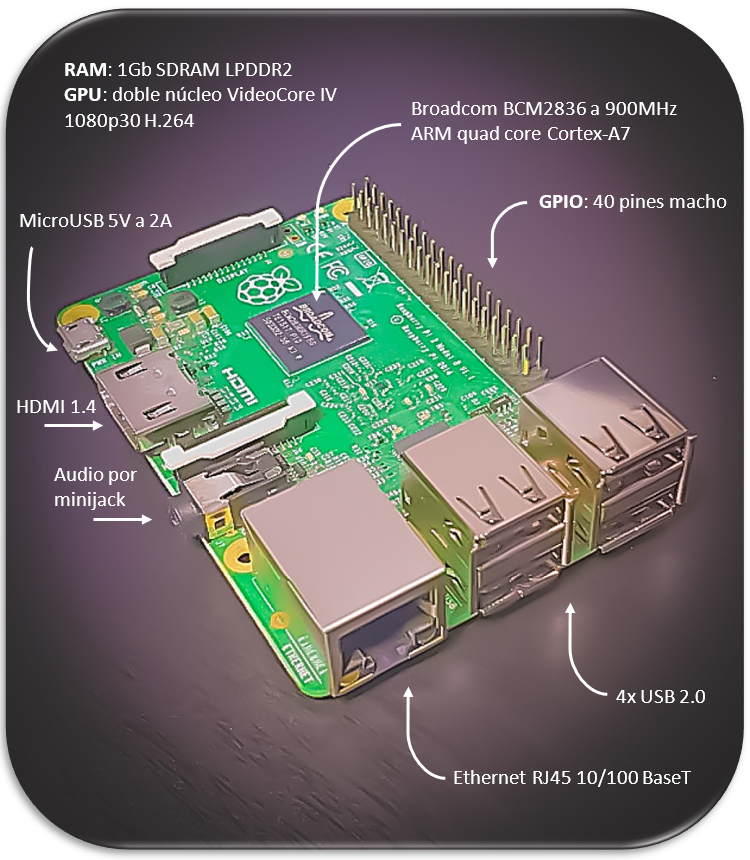
\includegraphics[width=.7\textwidth]{img/fotos/RbP_bueno.PNG}
\caption[Componentes Raspberry Pi]{Componentes Raspberry Pi.} \label{Img:3.RaspberryPi}
\end{figure}


Existen tres tipos de puertos GPIO en Raspberry Pi

Podemos ver los GPIO de la Raspberry Pi en la imagen~\ref{Img:3.RaspberryPi}, y también, la imagen~\ref{Img:3.GPIOReadAll} del comando <<gpio readall>> dentro de RasperryPi OS, donde podemos ver las numeraciones física, BCM y GPIO de los pines de la placa.

\begin{figure}[h]
    \centering
    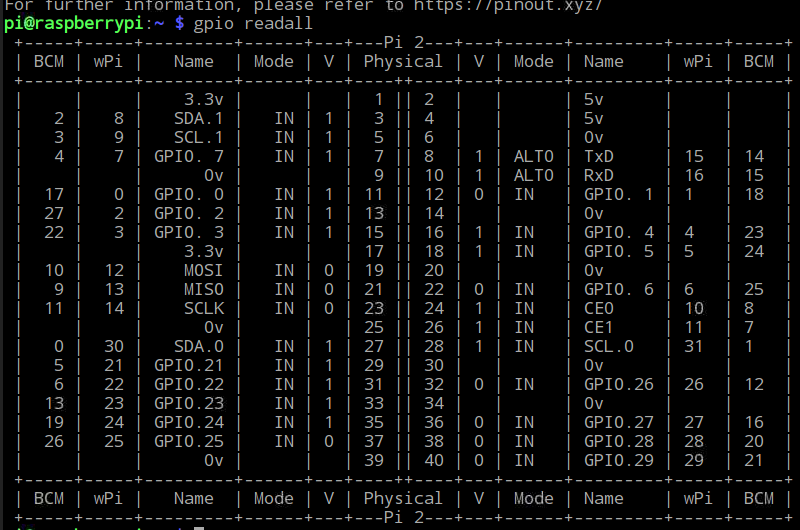
\includegraphics[width=.84\textwidth]{img/fotos/gpioReadall.png}
    \caption[Salida comando gpio readall]{Salida comando gpio readall.} \label{Img:3.GPIOReadAll}
\end{figure}


\section{API}\label{concepto:API}
Es el acrónimo de ‘Application Programming Interfaces’ que, traducido al castellano significa ‘Interfaz de Programación de Aplicaciones’. Estas interfaces nos sirven para realizar desarrollos. En nuestro caso utilizamos la información obtenida de Latitud y Longitud así como las temperaturas del día siguiente.
En el proyecto, accedemos a una URL como esta ~\url{http://ip-api.com/json/?fields=country,regionName,city,lat,lon,isp,query}, obteniendo los valores de país, región, ciudad, latitud, longitud, ISP y dirección IP.
Estos valores, podemos recogerlos directamente desde Python en formato json~\cite{misc:Json}, como podemos ver en el apartado~\ref{4:JSON}.

Otro ejemplo de API podemos verlo en Telegram, ya que utilizaremos su API orientada a crear bots para poder interactuar con nuestro sistema domótico. Podemos ver como funciona la API de Telegram con un bot programado por nosotros dependiendo de una Raspberry Pi en la imagen~\ref{Img:3.FuncionamientoBot}, que es la misma arquitectura que se ha utilizado en el proyecto.

\begin{figure}
    \centering
    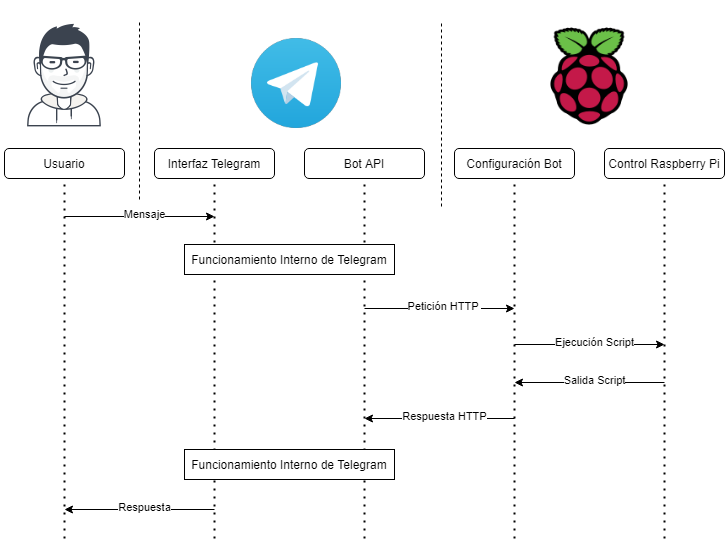
\includegraphics[width=1.\textwidth]{img/Diagramas/FuncionamientoBot.png}
    \caption[Funcionamiento Bot]{Funcionamiento Bot de Telegram con Raspberry Pi.} \label{Img:3.FuncionamientoBot}
\end{figure}

\section{Aplicación de mensajería multiplataforma}\label{concepto:AppMensajería}
Una aplicación de mensajería multiplataforma, es un software que nos permite enviar mensajes entre diferentes nodos o equipos, que utilizan este software, desde múltiples plataformas o sistemas.
Telegram es una de éstas aplicaciones de mensajería multiplataforma. Esta plataforma dispone de APIs a disposición de los usuarios que éstos pueden programar y poner a su propia disposición.
Podemos visitar la página web de la aplicación de mensajería en~\url{https://telegram.org/}.

\subsection{Bot de Telegram}\label{concepto:botTelegram}
Un bot, es un programa que permite simular una conversación en ciertos aspectos. Uno de estos aspectos puede ser enviarle órdenes para que las ejecute o nos brinde información de algún tipo. Como ejemplo, podemos ver plasmados ambos ejemplos en el bot que se ha desarrollado para el presente proyecto: podemos solicitarle al bot que ejecute acciones como el recopilado de datos o el envío de órdenes a los periféricos; y también que nos envíe información como puede ser una tabla informativa con las temperaturas por horas del día siguiente.

\section{Json}\label{concepto:JSON}
{Json~\cite{misc:Json}}, es el acrónimo en inglés de ‘JavaScript Object Notation’ y es un formato específico del que nos servimos para almacenar la información de forma estructurada mediante etiquetas <<key>> y etiquetas <<value>> del siguiente modo:

\begin{lstlisting}[language=json,firstnumber=0,basicstyle=\small ]
{
    "country":"Spain", 
    "regionName":"Madrid", 
    "city":"Getafe"
}
\end{lstlisting}

En ella, podemos ver que las etiquetas <<key>> son las que están a la izquierda de los dos puntos y las etiquetas de la derecha son las <<value>>. Tenemos un ejemplo real en el punto \ref{5.TelegramBot} del presente proyecto.

\section{RETB}\label{concepto:RETB}
Es el acrónimo de Reglamento electrotécnico para baja tensión y en él se recoge la normativa eléctrica aplicable en domicilios.
Esta norma acaba de ser actualizada y podemos disponer de la información en páginas oficiales como puede ser el BOE~\cite{manual:REBT}.
Del documento ICT-BT-21~\cite{manual:ICT-BT-21} podemos extraer información para realizar las instalaciones eléctricas de nuestro sistema domótico como el número máximo de cables a introducir por un tubo eléctrico.

\section{Normativa de ICT}\label{concepto:Normativa_ICT}
Como figura en el \textit{BOE 143, de 16 de junio de 2011, El Reglamento regulador de las infraestructuras comunes de telecomunicaciones para el acceso a los servicios de telecomunicación en el interior de las edificaciones, aprobado por el Real Decreto 346/2011, de 11 de marzo}:
Debemos regirnos por esta normativa a la hora de hacer cualquier instalación de comunicaciones nueva dentro de domicilios.
Podemos informarnos y ampliar información en la publicación en la sección de ICT en el BOE~\cite{manual:ICT}.

Por otro lado, disponemos de guías para instaladores con dibujos y tablas que facilitan la comprensión, como puede ser la documentación que publica Televés~\cite{manual:ICT-Televes}. De este punto, obtendremos la norma para introducir cableado ICT~\cite{manual:ICT} conforme a norma.

Tras hacer un estudio en mi domicilio, no necesitaré utilizar la normativa de ICT~\cite{manual:ICT} porque toda la instalación se realizará mediante canales eléctricos, pero está bien conocer la norma para, en caso de necesitarla, poder hacer uso de ella correctamente.

\section{Cableado estructurado}\label{concepto:Cableado_estructurado}
El establecimiento de un sistema de cableado estructurado consiste en la organización de los cables en un recinto conforme a una norma y constituye el nivel básico de cualquier red de comunicaciones.
Al contar y cumplir con este estándar nos damos cuenta de que tendremos instalaciones limpias, uniformes, seguras y escalables, facilitando la supervisión, el mantenimiento y posibles migraciones de tecnologías.
Un sistema de cableado genérico dispone de tres subsistemas, Troncal, de Edificio y Horizontal. En nuestro proyecto únicamente trataremos con el subsistema horizontal.

En este proyecto no contaremos con un gran número de cables, pero no está de más realizar una instalación lo más correctamente posible con unas normas de referencia

\section{WiFi}\label{concepto:WIFI}
Es una tecnología de comunicaciones de forma inalámbrica o <<Wireless>>. WiFi es el acrónimo traducido de <<Fidelidad Inalámbrica>> que procede del inglés <<Wireless Fidelity>>.
Estas tecnologías inalámbricas se rigen por la norma \underline{IEEE 802.11}~\cite{manual:IEEE802.11}.
En la web oficial del organismo podremos comprobar qué estándares dentro del 802.11 están vigentes y cuáles no.

\section{Tipos de cableado de datos}\label{concepto:UTP}
Es un tipo de cableado de datos que se compone de 4 pares de cables sin apantallar que están albergados dentro de una camisa de PVC.

Existen diferentes tipos de cables de datos: UTP, STP, FTP:
\begin{itemize}
\item Los cables \textbf{UTP} (del ingles <<Unshielded Twisted Pair>> o <<Par trenzado no apantallado>>) no disponen de protección ante interferencias electromagnéticas. Ver imagen~\ref{Img:CablesDatos}.



\item Los cables \textbf{FTP}(del inglés <<Foiled Twisted Pair>> o <<Par trenzado con pantalla global>>) disponen de una pantalla global contra interferencias electromagnéticas dentro de la camisa de PVC que recoge los 4 pares destinados a transmisión de datos. Ver imagen~\ref{Img:CablesDatos}.



\item Los cables \textbf{STP}(del inglés <<Shielded Twisted Pair>> o <<Par trenzado apantallado>>) disponen de una pantalla contra interferencias electromagnéticas por cada par de cables pero, además, también cuentan con una malla metálica exterior. Ver imagen~\ref{Img:CablesDatos}.


\end{itemize}
En nuestro caso utilizaremos UTP puesto que no necesitamos un apantallamiento ya que no transmitiremos datos y tampoco tendremos un alto grado de interferencias.

\capitulo{4}{Técnicas, herramientas y componentes}

Durante el proyecto se han utilizado diferentes tecnologías, herramientas y componentes que son imprescindibles y necesitan conocerse antes de continuar con el proyecto. Para optar por éstos y no por otros, se ha realizado una valoración que queda plasmada en este apartado a modo de justificación.

\section{Entorno Software}
\subsection{Raspbian (Distribución Linux)}
Como he comentado anteriormente, pretendo correr una distribución Linux en nuestro microPC. Las placas Raspberry Pi disponen de unas distribuciones de Linux desarrolladas expresamente para su hardware desde la Raspberry Pi Foundation. De esta manera conseguimos que el entorno esté diseñado para el hardware donde será ejecutado incluyendo, además, utilidades preinstaladas para explotarlas más fácil y eficientemente. Una de estas distribuciones optimizadas y orientadas a estas placas es Raspbian~\cite{misc:RbPWeb} o Raspberry Pi OS, que incluye software orientado a la educación, programación y otras de uso general. Algunas de estas aplicaciones son Python~\cite{misc:Python} (Lenguaje de programación que pretende que se desarrolle cógigo de una forma sencilla, rápida, poco costosa y legible), Scratch~\cite{misc:Scratch}(Simulador amigable para aprender programación.) o Java\cite{misc:Java}(Lenguaje de programación multiplataforma que utiliza una máquina virtual transparente para el usuario para ejecutarse), entre otros.

\subsection{Entorno de desarrollo Bash}
\begin{itemize}
    \item \textbf{Herramientas valoradas:} \href{https://www.freebsd.org/cgi/man.cgi?query=vi&sektion=1}{Vi}, \href{https://www.vim.org/}{Vim}, \href{https://www.nano-editor.org/}{Nano}.
    \item \textbf{Herramienta elegida:} \href{https://www.nano-editor.org/}{Nano}.
\end{itemize}

Nuestro Sistema Operativo Raspbian\cite{misc:RbPWeb}, al ser una distribución de Linux~\cite{misc:Linux}, dispone de líneas de comandos, procesadores de texto plano y editores de texto integrados. Éste es un editor de textos básico que facilita la interacción con él pese a que Vi o Vim son mucho más potentes.

\subsection{Entorno de desarrollo Python}
\begin{itemize}
    \item \textbf{Herramientas valoradas:} \href{https://www.jetbrains.com/es-es/pycharm/}{Jetbrains PyCharm} y \href{https://jupyter.org/}{Jupyter Notebook}.
    \item \textbf{Herramienta elegida:} \href{https://jupyter.org/}{Jupyter Notebook}.
\end{itemize}

Jupyter Notebook es un entorno de desarrollo interactivo y open source, basado en cuadernos que estructuran el código pudiendo ejecutarlo todo o parte. Dispone de una interfaz limpia, ligera e interactiva que nos permite programar en 40 lenguajes, incluyendo Python~\cite{misc:Python}.

\section{Control de datos}
\subsection{Web Scraping}
Es una técnica utilizada para extraer información de una página web utilizando las etiquetas de que dispone el propio lenguaje interpretado de HTML (del inglés <<HyperText Markup Language>> o lenguaje de marcas de hipertexto) para organizar elementos dentro de una página web, de forma que se introduce dentro de una etiqueta y subetiquetas hasta llegar al contenido del elemento requerido. Podemos entenderlo como si fueran contenedores lógicos configurables.
En nuestro caso, podremos utilizarlo desde Python~\cite{misc:Python} sirviéndonos de la librería <<beautifulsoup>> siempre que necesitemos obtener información de una página web.

\subsection{APIS}
\begin{itemize}
    \item \textbf{API situación geográfica}
\end{itemize}
En primer lugar estuve haciendo pruebas con la API de \url{www.ifconfig.me/ip} que devuelve la provincia en la que se encuentra tu IP pública pero quería una información más precisa ya que no tendremos la misma temperatura en El Escorial que en Aranjuez. Por ello, opté por \url{http://ip-api.com} que sí obtiene correctamente la ciudad desde la que nos conectamos.

\begin{itemize}
    \item \textbf{API Tiempo}
\end{itemize}
Al principio probé la API de \url{www.weatherapi.com} pero me entregaba únicamente la hora de salida y puesta del sol, lo cual es correcto para el control básico de las persianas pero quería llevar el proyecto más allá obteniendo además, una previsión de las temperaturas para el día siguiente pudiendo trabajar con ésta haciendo gráficos y poder decidir si encenderemos la calefacción o no. Y, por ello, opté por probar con la API de \url{www.climacell.co} que además, aseguran que es un 60\% más fiable que otras APIS ya que obtiene información de teléfonos móviles, cámaras y otros servicios online.

\subsection{json}
La librería json~\cite{misc:Json} para Python~\cite{misc:Python} y Python v3 nos permite, entre otros, parsear el código json~\cite{misc:Json} de archivos mediante la estructura de \textit{key:value}. En nuestro caso, tras obtener información de las APIs trataremos dicha información como json~\cite{misc:Json} gracias a su librería para Python~\cite{misc:Python}.

\section{Técnicas manuales}

\subsection{Tirada de cable con guía pasacables}
El procedimiento a seguir es el siguiente:
\begin{enumerate}
        \item Se abren las tapas de dos cajas de derivación próximas.
        \item Se introduce una guía pasacables (herramienta plástica con la forma de cuerda para introducir cables por canalizaciones) por el extremo de uno de los tubos dentro de la caja hasta llegar al otro extremo.
        \item Se asegura el cable a uno de los extremos de la guía pasacables.
        \item Se tira del otro extremo de la guía pasacables hasta conseguir sacar el cable por éste.
\end{enumerate}

\section{Metodologías}
\subsection{Scrum}
Scrum\cite{manual:Scrum} es un marco de trabajo para el desarrollo de software mediante la metodología ágil en el que se busca realizar un trabajo colaborativo de desarrollo incremental. Se aplica una metodología basada en milestones y sprints de forma iterativa.

\subsection{Modularidad}
Utilizaremos la modularidad para subdividir la aplicación en pequeños subprogramas que tienen una pequeña funcionalidad. De esta manera es más fácil detectar errores y escalar el proyecto. Además, teniendo clara la entrada y salida de cada uno de los módulos se pueden lanzar pruebas a cada uno de los módulos para comprobar su correcto funcionamiento mejorando, también, el mantenimiento.

\section{Entorno de desarrollo del Proyecto}

\subsection{Control de versiones o CVS, Concurrent Versioning System}
\begin{itemize}
    \item \textbf{Herramientas valoradas:} \href{https://git-scm.com/}{Git}, \href{https://subversion.apache.org/}{SVN}.
    \item \textbf{Herramienta elegida:} \href{https://git-scm.com/}{Git}.
\end{itemize}

Git es un software destinado al control de versiones software en el que se registran los cambios producidos en el mismo, facilitando la integración de código por parte de cualquiera de los integrantes del proyecto.
La diferencia más notable entre ellos es que Git es distribuido y SVN es un sistema centralizado. Significa que Git nos permite disponer de una copia en cada uno de los equipos desde los que se trabaje haciendo un clonado del repositorio, mientras que en SVN se trabaja en la nube.

\subsection{Hosting del Repositorio}
\begin{itemize}
    \item \textbf{Herramientas valoradas:} \href{https://github.com/}{Github} y \href{https://bitbucket.org/product/}{Bitbucket}.
    \item \textbf{Herramienta elegida:} \href{https://github.com/}{Github}.
\end{itemize}

Ambas opciones de hosting de repositorios funcionan de forma similar aunque GitHub incorpora opciones como la revisión de código, Kanban, Wikis o tableros entre otros que me han hecho decantarme por esta opción.
Ésta, es la plataforma principal de trabajo, que a su vez es una red social de código donde cualquiera puede contribuir en proyectos públicos y Open Source.


\subsection{Gestión del proyecto}
\begin{itemize}
    \item \textbf{Herramientas valoradas:} \href{https://teams.microsoft.com/}{MS.Teams}, \href{https://www.zenhub.com/}{ZenHub}, \href{https://github.com/}{GitHub Projects}, \href{https://www.zenhub.com/}{Trello}, \href{https://www.atlassian.com/es/software/jira}{Jira}, \href{https://www.board.com/es#gref}{Board}, \href{https://monday.com/lang/es/}{Monday}, \href{https://zube.io/}{Zube}, \href{https://clubhouse.io/}{Clubhouse}.
    \item \textbf{Herramienta elegida:} \href{https://www.zenhub.com/}{ZenHub}.
\end{itemize}

Es la única solución de colaboración en equipo integrada en GitHub y nos permite planificar hojas de ruta, generar informes, gestionar con Kanban, gestión ágil del proyecto mostrando la situación del proyecto para conseguir aumentar la productividad del equipo.

\subsection{Editor del proyecto}
\begin{itemize}
    \item \textbf{Herramientas valoradas:} \href{https://atom.io/}{Atom}, \href{https://code.visualstudio.com/}{Visual Studio Code}, \href{https://www.sublimetext.com/}{Sublime}.
    \item \textbf{Herramienta elegida:} \href{https://atom.io/}{Atom}.
\end{itemize}

Es un editor de código y texto creado por GitHub integrando las funciones de Git y GitHub, lo que nos facilita trabajar en nuestro equipo y replicar los cambios en Git, GitHub y ZenHub. Además, es un software multiplataforma, licencia open source, completamente personalizable, con temas y múltiples plugins, autocompletado y fácil navegación.
En este proyecto se utilizará para publicar las actualizaciones del proyecto.



\subsection{Dibujos, diagramas y planos}
\begin{itemize}
    \item \textbf{Herramientas valoradas:} \href{https://fritzing.org/}{Fritzing}, \href{https://support.microsoft.com/es-es/windows/obtener-microsoft-paint-a6b9578c-ed1c-5b09-0699-4ed8115f9aa9}{Paint, Paint3D}, \href{https://www.adobe.com/es/products/photoshop.html}{Photoshop}, y \href{www.draw.io}{Draw.io}.
    \item \textbf{Herramienta elegida:} \href{https://fritzing.org/}{Fritzing} y \href{www.draw.io}{Draw.io}.
\end{itemize}
Realmente no pude decidirme por entre Fritzing y draw.io puesto que cada uno está orientado a un tipo de tarea:

Fritzing es un software con licencia Open Source\cite{misc:OpenSource} que nos permite realizar material electrónico fácilmente, aunque desde hace algún tiempo debemos hacer un pequeño desembolso por la descarga. En mi caso con el fin de entregar diagramas de calidad los haré con este software.

Por otro lado, Draw.io está pensado para hacer planos y dibujos que no están orientados a la electrónica, por lo que es muy útil para hacer otro tipo de diagramas.

\subsection{Procesador de textos \LaTeX}
\begin{itemize}
    \item \textbf{Herramientas valoradas:} \href{https://www.latex-project.org/}{\LaTeX}, \href{https://www.microsoft.com/es-es/microsoft-365/word}{MS Word}, \href{https://www.sublimetext.com/}{Sublime}, \href{https://www.overleaf.com/}{Overleaf}.
    \item \textbf{Herramienta elegida:} \href{https://www.latex-project.org/}{\LaTeX} y \href{https://www.overleaf.com/}{Overleaf}.
\end{itemize}
\LaTeX{} es un editor de textos open source\cite{misc:OpenSource} con alta calidad tipográfica que trabaja con etiquetas permitiéndonos separar nuestro contenido del estilo del mismo. Para escribir el proyecto en \LaTeX utilizaré Overleaf por su capacidad de compilado instantáneo de forma que se puede comprobar como modificas la redacción en tiempo real.

\section{Entorno físico}
\subsection{RaspberryPi}
En nuestro proyecto tendremos el control de la instalación domótica desde una Raspberry Pi\cite{misc:RbPWeb}. 
Para dar un enfoque muy general, podemos decir que las placas RaspberryPi~\cite{misc:RbPWeb} son microordenadores que disponen de poca potencia si las comparamos con equipos usuales, pero disponen de suficiente potencia para llevar a cabo este tipo de proyectos.

Se diseñaron en su origen por la RaspBerry Pi Foundation~\cite{misc:RbPWeb} en el Reino Unido para dotar de equipos informáticos a los centros de estudios a un bajo coste, pero el proyecto ha evolucionado para poder desarrollar, además, otras muchas tareas como puede ser nuestro caso, que la utilizaremos como ‘núcleo’ de toda nuestra instalación domótica y, será donde configuremos todo el entorno domótico de la vivienda.
Estas placas pueden ejecutar con agilidad distribuciones Linux~\cite{misc:Linux} y, desde sus distribuciones podemos interactuar con sus famosos <<GPIO>>, ver imagen ~\ref{Img:Especificaciones RBP2B}

\begin{figure}
    \centering
    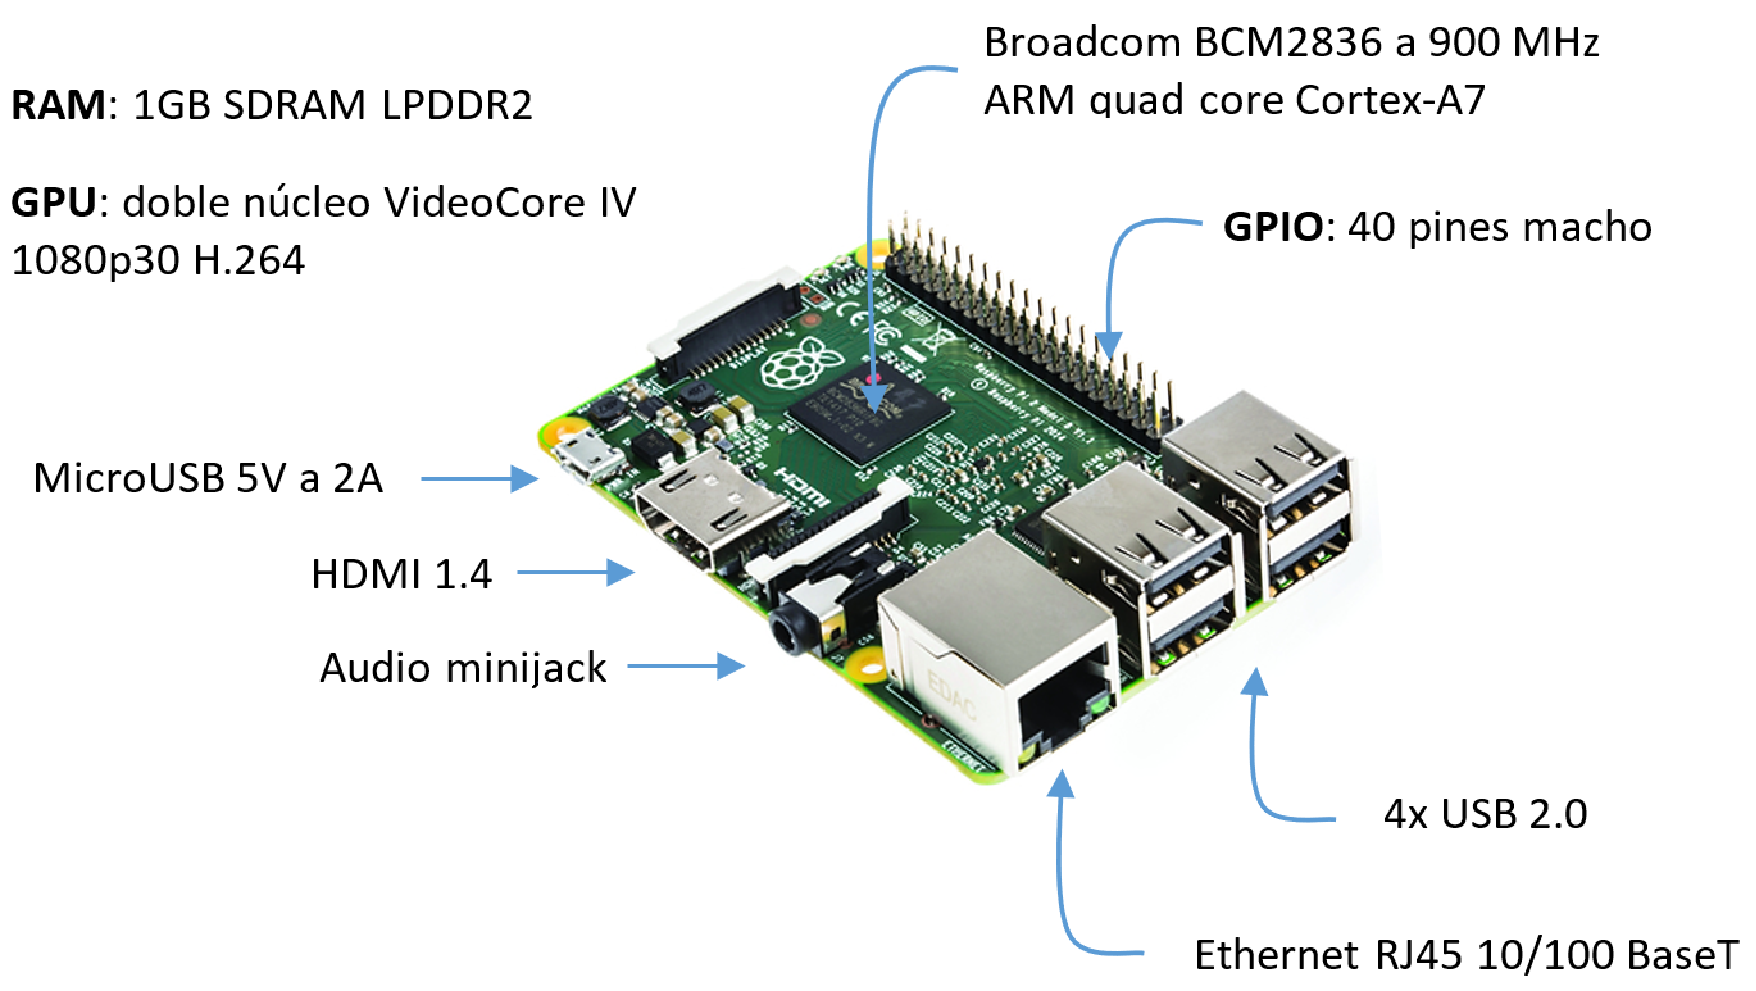
\includegraphics[width=\textwidth]{img/RBP2B.pdf}
    \caption[Especificaciones de Raspberry Pi 2B]{Especificaciones de Raspberry Pi 2B. Imagen de \url{https://raspberryparatorpes.net} modificada por el autor del TFG~\cite{wiki:Creative}. }\label{Img:Especificaciones RBP2B}
\end{figure}

\subsection{Relé}
Es un dispositivo electromagnético que desempeña la misma función de un interruptor, es decir, con nuestros relés, dejaremos pasar la energía eléctrica, o no, a nuestros dispositivos. Los relés se activan mediante impulsos eléctricos que abren o cierran el circuito según se predisponga. Podemos verlo en la imagen~\ref{Img:Rele1}.
\begin{figure}
    \centering
    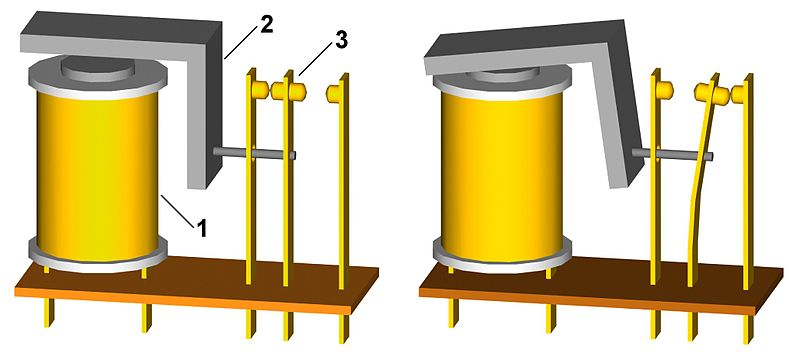
\includegraphics[width=\textwidth]{img/Rele_1.jpg}
    \caption[Estructura interna de un relé]{Estructura interna de un relé. Imagen de \url{https://commons.wikimedia.org/}\cite{manual:GNU}} \label{Img:Rele1}
\end{figure}

\subsection{Placa de Pruebas o ProtoBoard}
Es un tablero electrónico para realizar pruebas. Protoboard es la agrupación de los términos ingleses “prototype board”.
Esta protoboard la he instalado para poder hacer fácilmente el interconexionado entre los cables que llegan de los relés y los que van a la Raspberry Pi, evitando posibles tirones y movimiento de cables a la hora de hacer alguna manipulación.

Éstas, disponen de tres zonas diferenciadas(Ver imagen ~\ref{Img:Protoboard}):

\begin{itemize}
    \item \textbf{Canal Central}: Está situada en el medio de la placa y es donde se colocan los circuitos.
    \item \textbf{Buses}: Se sitúan en los extremos de la placa y disponen de dos líneas:
        \subitem \textbf{Línea roja}: Bus positivo o de voltaje.
        \subitem \textbf{Línea azul}: Bus negativo o de tierra.
    \item \textbf{Pistas}: Se sitúan en la zona central de la placa y, conducen en sentido contrario de las líneas rojas y azul.
\end{itemize}

\begin{figure}
    \centering
    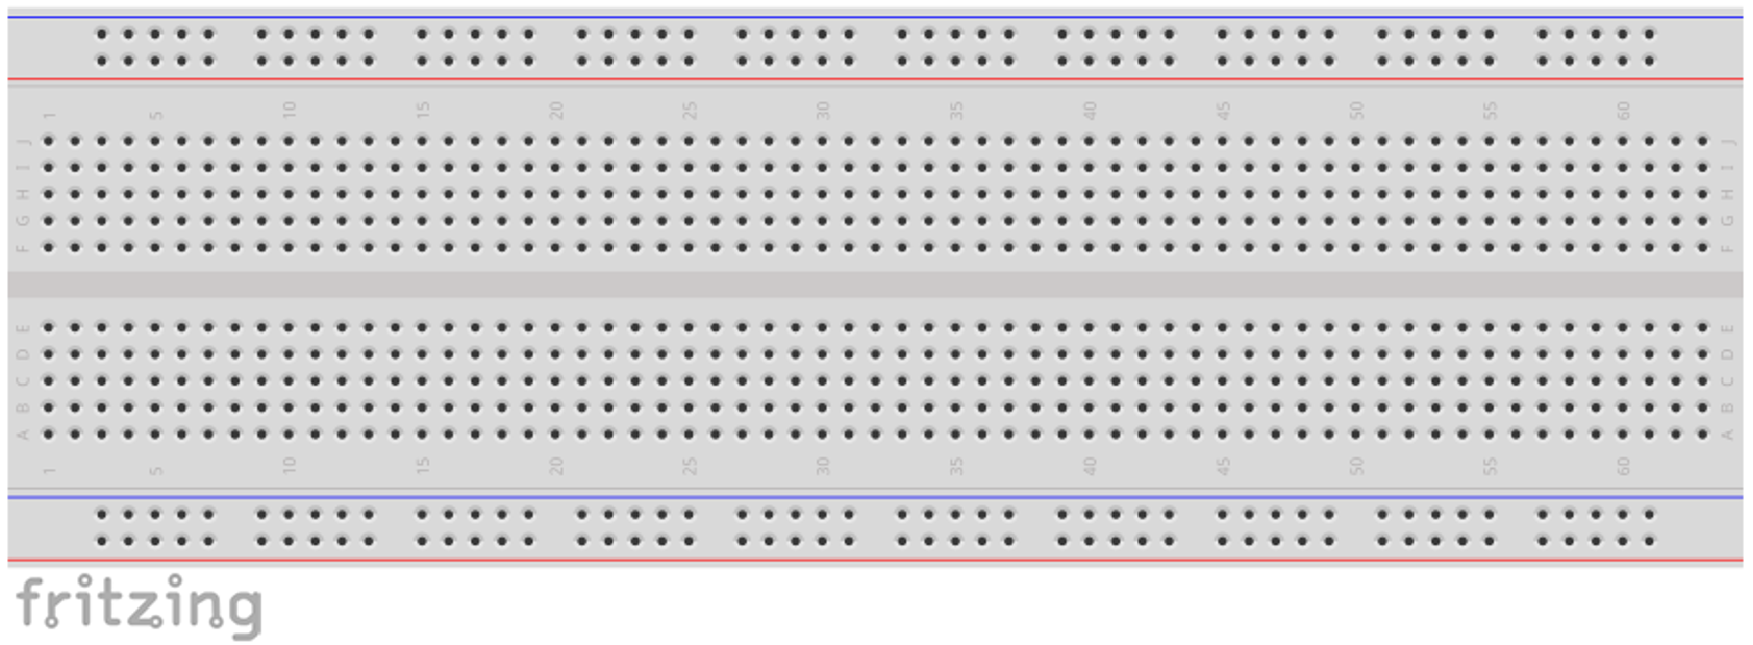
\includegraphics[width=0.9\textwidth]{img/protoboard.pdf}
    \caption{Imagen de una placa <<protoboard>>. } \label{Img:Protoboard}
\end{figure}

\subsection{Router}
Es un dispositivo que nos permite interconectar diferentes redes de datos. En mi caso dispongo de un router con WiFi integrado para poder dotar a la Raspberry Pi de salida a Internet.

\section{Plataforma de interacción}
\begin{itemize}
    \item \textbf{Herramientas valoradas:} \href{https://telegram.org/}{Telegram}, \href{https://palletsprojects.com/p/flask/}{Flask}.
    \item \textbf{Herramienta elegida:} \href{https://telegram.org/}{Telegram}.
\end{itemize}
Para finalizar el proyecto con una interfaz de interacción se valoraron las opciones de desaroolar un página web ligera o una aplicación de mensajería.
En primer lugar se propuso hacer una aplicación en Flask pero pareció más novedoso y potente hacer un Bot de Telegram de forma que podamos interactuar con él y enviarnos información bajo demanda. Además, se elimina el buscar hosting y dominio para albergar los servicios propios del sistema domótico abaratando más los costes, además de incrementar la seguridad al utilizar mensajería cifrada.


\capitulo{5}{Aspectos relevantes del desarrollo del proyecto}

Este apartado pretende recoger los aspectos más interesantes del desarrollo del proyecto, comentados por los autores del mismo.
Debe incluir desde la exposición del ciclo de vida utilizado, hasta los detalles de mayor relevancia de las fases de análisis, diseño e implementación.
Se busca que no sea una mera operación de copiar y pegar diagramas y extractos del código fuente, sino que realmente se justifiquen los caminos de solución que se han tomado, especialmente aquellos que no sean triviales.
Puede ser el lugar más adecuado para documentar los aspectos más interesantes del diseño y de la implementación, con un mayor hincapié en aspectos tales como el tipo de arquitectura elegido, los índices de las tablas de la base de datos, normalización y desnormalización, distribución en ficheros3, reglas de negocio dentro de las bases de datos (EDVHV GH GDWRV DFWLYDV), aspectos de desarrollo relacionados con el WWW...
Este apartado, debe convertirse en el resumen de la experiencia práctica del proyecto, y por sí mismo justifica que la memoria se convierta en un documento útil, fuente de referencia para los autores, los tutores y futuros alumnos.

\capitulo{6}{Trabajos relacionados}
\begin{comment}
Este apartado sería parecido a un estado del arte de una tesis o tesina. En un trabajo final grado no parece obligada su presencia, aunque se puede dejar a juicio del tutor el incluir un pequeño resumen comentado de los trabajos y proyectos ya realizados en el campo del proyecto en curso. 
\end{comment}

\capitulo{6}{Trabajos relacionados}

Desde la aparición de elementos electrónicos accesibles y asequibles se ha intentado, con mayor o menor fortuna, generar sistemas que nos ayuden en nuestro día a día. A continuación se exponen proyectos con objetivos similares.

\section{Comparativa con otros proyectos}
En este apartado mostraré otras opciones de acometer un proyecto similar y compararé los principales puntos de éstos con el presente proyecto para poder tener una visión global entre estas opciones.

\section{Presentación de los proyectos}
\subsection{Interacción remota para elementos de un hogar mediante una red de sensores actuadores}
Se trata de un proyecto de control domótico que se centra en un conjunto de sensores instalados en el domicilio utilizando nodos intermedios para realizar el control de los dispositivos finales y la comunicación con los sensores.

En la tabla ~\ref{tabla_Interacción} podemos ver algunas características de este proyecto.
En las tablas se representará con la primera palabra del nombre del proyecto: "Interacción".

\begin{table}[H]
\centering
\begin{tabular}{lccc}
\toprule
Características & Interacción  \\
\midrule
Proyecto libre                          & \cellcolor{green!25} {$\checkmark$}\\
No precisa montar servicios             &  \cellcolor{red!25} {$\times$}  \\
No requiere lenguajes no nativos en el SO & \cellcolor{red!25} {$\times$} \\
Obtiene información externa contrastada & \cellcolor{red!25} {$\times$} \\
Interacción multiplataforma             & \cellcolor{green!25} {$\checkmark$} \\
No necesita nodos intermedios           & \cellcolor{red!25} {$\times$} \\
Cableado entre elementos                & \cellcolor{red!25} {$\times$} \\
WiFi entre elementos                    & \cellcolor{green!25} {$\checkmark$} \\
\bottomrule
\end{tabular}
\caption{Comparativa de las características de los proyectos.}
\label{tabla_Interacción}
\end{table}

\subsection{Diseño e implementación de un sistema domótico basado en Raspberry Pi}
Se trata de un proyecto de control domótico que se centra en un conjunto de sensores instalados en el domicilio.

\begin{itemize}
    \item Url del trabajo: \url{https://e-archivo.uc3m.es/bitstream/handle/10016/26313/TFG_Hector_Santos_Senra.pdf?sequence=1&isAllowed=y}
\end{itemize}

En la tabla ~\ref{tabla_Diseño} podemos ver algunas características de este proyecto.
En las tablas se representará con la primera palabra del nombre del proyecto: "Diseño".
\begin{table}[H]
\centering
\begin{tabular}{lccc}
\toprule
Características & Diseño  \\
\midrule
Proyecto libre                          & \cellcolor{red!25} {$\times$} \\
No precisa montar servicios             & \cellcolor{red!25} {$\times$} \\
No requiere lenguajes no nativos en el SO  & \cellcolor{red!25} {$\times$} \\
Obtiene información externa contrastada & \cellcolor{red!25} {$\times$} \\
Interacción multiplataforma             & \cellcolor{green!25} {$\checkmark$} \\
No necesita nodos intermedios           & \cellcolor{green!25} {$\checkmark$} \\
Cableado entre elementos                & \cellcolor{green!25} {$\checkmark$} \\
WiFi entre elementos                    & \cellcolor{red!25} {$\times$} \\
\bottomrule
\end{tabular}
\caption{Comparativa de las características de los proyectos.}
\label{tabla_Diseño}
\end{table}

\section{Fortalezas y debilidades del proyecto}

Las principales fortalezas del proyecto son:

\begin{itemize}
\tightlist
\item
    Éste es un proyecto que cualquiera puede implementar fácilmente en su domicilio haciendo una copia local del repositorio y haciendo unas sencillas configuraciones en el archivo de configuración.
    
\item
    En este proyecto se ha tenido en cuenta la eficiencia de recursos y de consumo de la propia máquina Raspberry Pi\cite{misc:RbPWeb}, por lo que no se han incluido servicios extraordinarios como puede ser un servidor de bases de datos o web, como sucede en otros proyectos. Se ha optado por incluir un bot que 'escucha' las órdenes y actúa conforme a un pequeño archivo de configuración y actúa contra la máquina utilizando los lenguajes nativos de la máquina. De esta manera, el gasto en cómputo es menor y también el utilizado en mantener los servicios en memoria, quedando recursos suficientes para continuar haciendo un uso normal de la máquina para cualquier otra tarea.
    Además, al no tener servidores levantados y con puertos de comunicaciones abiertos, aumentamos la seguridad de nuestra instalación.

\item
    Se ha procurado utilizar los lenguajes integrados de forma nativa en el Sistema Operativo para evitar posibles fallos de integración entre ellos y aumentando la fiabilidad del sistema. Estos son Python~\cite{misc:Python} y Bash~\cite{misc:Linux}. 
    
\item
    El sistema automatizado de nuestro proyecto se nutre de la información contrastable obtenida de API's reconocidas.
    
\item
    Se puede interactuar con el sistema domótico de varias formas. La más cómoda es mediante el bot de Telegram creado en exclusiva para controlar las funcionalidades principales de nuestro sistema domótico, aunque también se puede contectar de forma remota desde otra máquina mediante VNC~\footnote{VNC: "Virtual Network Computing", programa de control remoto de equipos informáticos basado en una estructura cliente-servidor} siempre que se esté en la misma red. Se puede interactuar con el bot mediante aplicaciones Android o IOs, o desde navegadores de uso extendido como Chrome, Firefox o Edge, entre otros.
    
\item
    No se necesitan elementos intermedios de ningún tipo, únicamente tenemos nuestra Raspberry Pi~\cite{misc:RbPWeb} y los actuadores o relés~\ref{Img:Rele1}. De esta manera evitamos posibles fallos de los elementos intermedios.
    \begin{comment}
        --> TODO: Esta situación podemos comprobarla en la imagen PLANO GENERAL DE LA INSTALACIÓN
    \end{comment}
    
\item
    Se ha preferido cablear la instalación para evitar que los elementos receptores puedan quedar en un estado no deseado así como evitar reconfigurar elementos ante cualquier posible cambio de alguno de los elementos como pueden ser el dongle WiFi~\ref{concepto:WIFI} o el router.
    También, al dejar libres los canales WiFi, evitamos contribuir a la actual saturación de frecuencias en los espectros de 2.4GHz y 5GHz~\cite{manual:IEEE802.11}.

\end{itemize}


Podemos ver en la tabla~\ref{tabla:comparativa-proyectos} de comparativa de proyectos lo anteriormente expuesto.

\begin{itemize}
\tightlist
\end{itemize}
\begin{table}[H]
\centering
\begin{tabular}{lccc}
\toprule
Características & SDI & Interacción & Diseño  \\
\midrule
Proyecto libre                          & \cellcolor{green!25} {$\checkmark$} & \cellcolor{green!25} {$\checkmark$} & \cellcolor{red!25} {$\times$} \\
No precisa montar servicios             & \cellcolor{green!25} {$\checkmark$} & \cellcolor{red!25} {$\times$} & \cellcolor{red!25} {$\times$} \\
No requiere lenguajes no nativos en el SO  & \cellcolor{green!25} {$\checkmark$} & \cellcolor{red!25} {$\times$} & \cellcolor{red!25} {$\times$} \\
Obtiene información externa contrastada & \cellcolor{green!25} {$\checkmark$} & \cellcolor{red!25} {$\times$} & \cellcolor{red!25} {$\times$} \\
Interacción multiplataforma             & \cellcolor{green!25} {$\checkmark$} & \cellcolor{green!25} {$\checkmark$} & \cellcolor{green!25} {$\checkmark$} \\
No necesita nodos intermedios           & \cellcolor{green!25} {$\checkmark$} & \cellcolor{red!25} {$\times$} & \cellcolor{green!25} {$\checkmark$} \\
Cableado entre elementos                & \cellcolor{green!25} {$\checkmark$} & \cellcolor{red!25} {$\times$} & \cellcolor{green!25} {$\checkmark$} \\
WiFi entre elementos                    & \cellcolor{red!25} {$\times$} & \cellcolor{green!25} {$\checkmark$} & \cellcolor{red!25} {$\times$} \\
\bottomrule
\end{tabular}
\caption{Comparativa de las características de los proyectos.}
\label{tabla:comparativa-proyectos}
\end{table}

Las principales debilidades del proyecto son:

\begin{itemize}
\tightlist
\item
    Hace falta cierta soltura a la hora de trabajar con el cableado UTP~\ref{4:guiaPasacables}.
\item
    Es necesaria una línea de datos para que se actualicen los parámetros de los scripts.

\end{itemize}

\capitulo{7}{Conclusiones y Líneas de trabajo futuras}
\begin{comment}
Todo proyecto debe incluir las conclusiones que se derivan de su desarrollo. Éstas pueden ser de diferente índole, dependiendo de la tipología del proyecto, pero normalmente van a estar presentes un conjunto de conclusiones relacionadas con los resultados del proyecto y un conjunto de conclusiones técnicas. 
Además, resulta muy útil realizar un informe crítico indicando cómo se puede mejorar el proyecto, o cómo se puede continuar trabajando en la línea del proyecto realizado. 
\end{comment}

Con este apartado concluye la memoria de este proyecto, desglosando cada uno de los objetivos superados en el mismo. Posteriormente se sugerirán algunas posibles líneas de trabajo futuras que puedan dar continuidad al proyecto consiguiendo una mejora notable.

\section{Conclusiones}
Una vez finalizado el proyecto, podemos concluir con las siguientes afirmaciones:
\begin{itemize}
\item Se ha conseguido crear un Sistema de Simulación de Presencia que funciona según las horas de luz del día. En cada jornada, el Sistema genera una consulta de forma automática obteniendo los parámetros de ubicación, y posteriormente, los parámetros de salida y puesta de sol. Seguidamente procesa los datos para controlar los diferentes elementos externos.

\item Además, se ha ampliado el Sistema de Simulación de Presencia con el Sistema Domótico que controla la caldera, las persianas y las luces. De esta manera, también controlamos a que hora se suben las persianas por las mañanas y se controla el encendido de la caldera. Esta parte es parcialmente automática ya que tenemos la opción de subir las persianas, tras el amanecer, a la hora que queramos.

\item Se ha conseguido dotar al sistema de un control instantáneo de las persianas. Este apartado beneficia a la hora de querer controlar una persiana de forma individual y en un intervalo de tiempo corto.

\item También, se han incluido órdenes informativas que funcionan a partir de la información recopilada porque no cuesta nada poder contar con la información recopilada de una forma limpia e instantánea siempre que la queramos. Además, se dibujan diariamente una gráfica con las temperaturas del día siguiente que también están a nuestra disposición siempre que solicitemos el envío de alguna de ellas

\item El sistema es autónomo de la ubicación en la que está instalado ya que obtiene su ubicación en cada consulta lo cual es necesario para poder obtener las temperaturas del día siguiente.

\item Se ha generado un bot para automatizar todo el proceso de comunicación con el Sistema Domótico Inteligente de forma que podemos interactuar con él desde cualquier lugar de una manera segura y minimizando el cómputo, los servicios activos y también los puertos abiertos.

\item El sistema, finalmente, funciona con un mínimo de instrucciones y programas en background, lo cual contribuye a un mínimo consumo energético y pone a disposición del usuario los recursos de la máquina para realizar otras tareas que se precisen.

\item Estoy satisfecho con la instalación física realizada en el domicilio, me parece profesional ya que sigue las líneas de las normativas legales vigentes por las que se rigen este tipo de instalaciones.

\item Otro punto muy satisfactorio es el de la mínima inversión acometida en el proyecto junto a una funcionalidad completa hacen que sienta que el dinero ha sido muy bien invertido ya que ha aumentado notablemente la comodidad y confortabilidad del domicilio. Además se nota que, ahora en invierno, la temperatura de la vivienda desciende más despacio al bajarse las persianas cuando anochece.

\item La única pega que le podría al proyecto es que al utilizar la versión 2B de la Raspberry Pi, algunas peticiones tardan unos segundos más de lo que me gustaría. Esto sucede cuando se le ordena que modifique la hora de subida de las persianas ya que debe abrir y modificar varios archivos, pero se soluciona con una versión más nueva de Raspberry Pi.

\end{itemize}


\section{Líneas de trabajo futuras}
El proyecto ha quedado bastante <<redondo>>, es decir, se ha generado una funcionalidad completa y se ha dado solución a una necesidad dentro de los parámetros que se esperaba. No obstante, el proyecto es susceptible de crecer para aumentar el confort y mejorar el Sistema Simulador de Presencia y el Sistema Domótico.

\begin{itemize}
\item El proyecto se centra únicamente en valores externos como son el Sol o la temperatura exterior. Se puede incluir un sensor de temperatura en la vivienda de forma que también se controle la calefacción siempre que la caldera esté encendida.

\item Al Sistema Simulador de Presencia podemos incluirle sonido. Una buena opción puede ser conseguir emitir un programa en streaming~\footnote{Retransmisión en directo.}, ya sea solo audio o también con vídeo.

\item Ya que hemos incluido Telegram y éste dispone de llamadas, podemos incluir un <<portero IP>> de forma que te llame a un usuario y puedas comunicarte con quien llame a la puerta. De esta manera no sólo simulas que estás en el domicilio sino que también sabes quién ha estado en tu puerta. Este portero puede ser sólo con voz o también con imagen.

\item Al mismo sistema, se le pueden incorporar unos sensores PIR para saber en que parte de la casa hay movimiento y disponer un control de luces o grabado de imágenes.

\item También se puede optar por crecer en la rama de seguridad añadiendo sensores de gas, agua y humo para y notifique las alertas.

\item Si se vive en un lugar con puerta de garaje individual, se puede programar para interactuar con ésta permitiendo el acceso con un mensaje.

\item Ante todas estas líneas de trabajo, quiero figurar la primera mejora que implementaré cuando sea posible. Esta será implementar un BUS para conectar los GPIO con cada uno de los cables que controlan los relés, soldando éstos al bus, y de esta manera eliminaríamos la protoboard.

\end{itemize}



\bibliographystyle{plain}
\bibliography{bibliografia}

\end{document}
